\documentclass{beamer}
\usetheme{Madrid}

\usepackage{listings}
\usepackage{graphicx}
\usepackage{amsmath}
\usepackage{xcolor}
\usepackage{pifont}

\setbeamertemplate{frametitle}[default][center]
\setbeamertemplate{footline}{}
\setbeamertemplate{navigation symbols}{}
\setbeamercovered{dynamic}

\title{Utilizing Crowd Intelligence for Online Detection of Emotional Distress}
\subtitle{Master's Thesis Presentation}
\author[Siddhant Goel]{Siddhant Goel\\{\small Advisor: Han Xiao\\Supervisor: Prof. Dr. Claudia Eckert}}
\institute{
Chair for IT Security\\
Technische Universit\"at M\"unchen
}
\date{\today}

\begin{document}
    \begin{frame}[plain]
        \titlepage
    \end{frame}
    
    \begin{frame}
        \frametitle{Outline}
        \begin{itemize}
            \item{
            Introduction
            \begin{itemize}
                \item{Backdrop}
                \item{Motivation}
                \item{Problem Definition}
            \end{itemize}
            }
            \pause
            \item{
            Theoretical Background
            \begin{itemize}
                \item{Machine Learning and Text Classification}
                \item{Support Vector Machines}
                \item{Ensemble Learning methods}
            \end{itemize}
            }
            \pause
            \item{Experiments}
            \item{System}
            \item{Conclusion and Future Work}
            \item{Q/A}
        \end{itemize}
    \end{frame}
    
    \begin{frame}
        \begin{center}
            \textbf{Introduction}
        \end{center}
    \end{frame}
    
    \begin{frame}
        \frametitle{Backdrop}
        \begin{block}{Depression and Suicide}
            \begin{itemize}
                \item{Nearly one million people die every year because of suicide}
                \item{Most people are between 15 to 29 years old}
            \end{itemize}
        \end{block}
        \pause
        \begin{block}{Social Media}
            \begin{itemize}
                \item{Rise of Twitter, Facebook, Reddit, Wordpress}
                \item{
                Sections of interest
                \begin{itemize}
                    \item{Reddit - ``/r/happy'' \footnote{\url{http://www.reddit.com/r/happy}} and ``/r/suicidewatch'' \footnote{\url{http://www.reddit.com/r/suicidewatch}}}
                    \item{Twitter - the entire website}
                \end{itemize}
                }
            \end{itemize}
        \end{block}
    \end{frame}
    
    \begin{frame}
        \frametitle{Backdrop}
        \begin{figure}
            \centering
            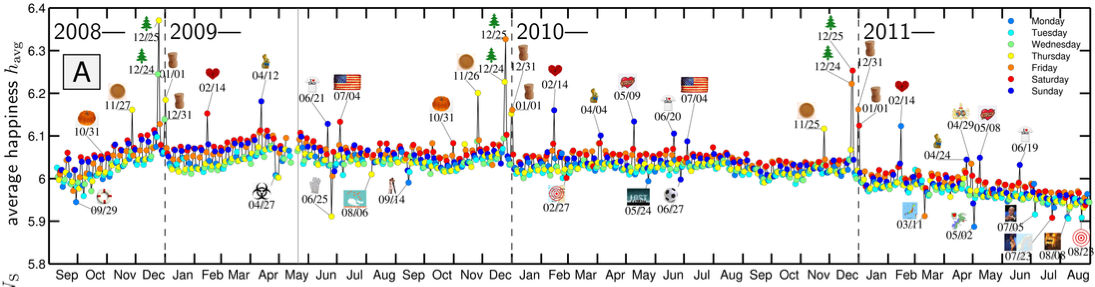
\includegraphics[width=\textwidth]{figures/twitter_happiness.png}
        \end{figure}
        \begin{itemize}
            \item{Study conducted in 2011}
            \item{46 billion words collected over 33 months}
            \item{Negativity on Twitter has been on the rise}
            \item{Words include \emph{death}, \emph{hate}, and even \emph{suicide}}
        \end{itemize}
    \end{frame}
    
    \begin{frame}
        \frametitle{Motivation}
        \begin{figure}
            \centering
            
\includegraphics[width=0.5\textwidth]{figures/twitter_kcs.png}
        \end{figure}
        \begin{itemize}
            \item{\textbf{Direct} - \emph{``thoughts of \textcolor{red}{suicide} make me happy''}, \emph{``I have a \textcolor{red}{rope around my neck}''}}
            \item{\textbf{Indirect} - \emph{``I \textcolor{red}{don't know} anything anymore''}, \emph{``\textcolor{red}{Need someone} to talk to''}}
            \pause
            \item{Some accounts have lots of followers, some don't}
            \item{Lives can be saved if there is a surveillance system of suicide}
            \item{Public sentiment information available on the web + No analysis possible = Disconnect}
        \end{itemize}
    \end{frame}
    
    \begin{frame}
        \frametitle{Problem Definition}
        \begin{block}{Experiments}
            Evaluate machine learning algorithms that can be used for identifying depressed emotions in pieces of text
        \end{block}
        \begin{block}{System}
            Build a web based system that can
            \begin{itemize}
                \item{tap into \textcolor{blue}{crowd intelligence} to incrementally improve the classifiers}
                \item{\textcolor{blue}{detect content} on the web that indicates that its author may be \textcolor{blue}{depressed or suicidal}}
            \end{itemize}
        \end{block}
    \end{frame}
    
    \begin{frame}
        \begin{center}
            \textbf{Theoretical Background}
        \end{center}
    \end{frame}
    
    \begin{frame}
        \frametitle{Machine Learning}
        \begin{itemize}
            \item{Algorithms that can learn from data}
            \item{Construct a model from a given dataset, and then perform the required task on another dataset}
            \pause
            \item{\textbf{Supervised learning} - Train the models on the training data, and predict on the test data}
            \item{\textbf{Unsupervised learning} - No distinction between training and test data}
        \end{itemize}
    \end{frame}
    
    \begin{frame}
        \frametitle{Text Classification}
        \begin{block}{Formal definition}
            Given a dataset $\{(\mathbf{x_n}, y_n)\}_{n = 1}^{N}$ containing N instances, where each instance $(\mathbf{x_n}, y_n)$ is of the form $[(x_{n, 1}, x_{n, 2}, ..., x_{n, D}), y_n]$, calculate the $y_n$ values.
        \end{block}
        \pause
        \begin{itemize}
            \item{Given some pieces of text, put unseen pieces of text into two or more categories}
            \item{\textbf{Supervised} - calculate $y_n$ of test data given information about $y_n$ from training data}
            \item{\textbf{Unsupervised} - calculate $y_n$ given only information about $\mathbf{x_n}$}
        \end{itemize}
    \end{frame}
    
    \begin{frame}
        \frametitle{Document Representation}
        \begin{columns}
            \visible<1->{
                \begin{column}{0.3\textwidth}
                    \begin{center}
                        \textbf{Text Corpus} \\
                        \textcolor{blue}{``I am happy today''} \\
                        and\\
                        \textcolor{red}{``I am not happy today, but I was happy yesterday''}
                    \end{center}
                \end{column}
            }
            \visible<2->{
                \begin{column}{0.05\textwidth}
                    $\rightarrow$
                \end{column}
            }
            \visible<3->{
                \begin{column}{0.3\textwidth}
                    \begin{center}
                        \textbf{Token dictionary}\\
                        ``I'': 1,\\
                        ``am'': 2,\\
                        ``happy'': 3,\\
                        ``today'': 4,\\
                        ``not'': 5,\\
                        ``but'': 6,\\
                        ``was'': 7,\\
                        ``yesterday'': 8\\
                    \end{center}
                \end{column}
            }
            \visible<4->{
                \begin{column}{0.05\textwidth}
                    $\rightarrow$
                \end{column}
            }
            \visible<5->{
                \begin{column}{0.3\textwidth}
                    \begin{center}
                        \textbf{Vector Space Representation}\\
                        \textcolor{blue}{\[1, 1, 1, 1, 0, 0, 0, 0\]}\\
                        and\\
                        \textcolor{red}{\[2, 1, 2, 1, 1, 1, 1, 1\]}\\
                    \end{center}
                \end{column}
            }
        \end{columns}
    \end{frame}
    
    \begin{frame}
        \frametitle{Support Vector Machines}
        \begin{itemize}
            \item{Fairly popular class of algorithms used for binary classification}
            \item{Given training data in some $D$ dimensional space, find a decision boundary (hyperplane) that separates the two classes}
            \pause
            \item{Hyperplane ($\mathbf{w} \cdot \mathbf{x} - b = 0$) should have maximum distance from any data point}
            \item{Solution for linear classifiers: $\mathbf{w} = \displaystyle \sum_{i = 1}^{S} \alpha_i\mathbf{x_i}$}
            \pause
            \item{Replace $\mathbf{x_i} \cdot \mathbf{x}$ with $k(\mathbf{x_i}, \mathbf{x})$ $\implies$ represents the dot product of two vectors in higher dimensions (kernel function)}
        \end{itemize}
    \end{frame}
    
    \begin{frame}
        \frametitle{Linear kernel SVM}
        \begin{figure}
            \centering
            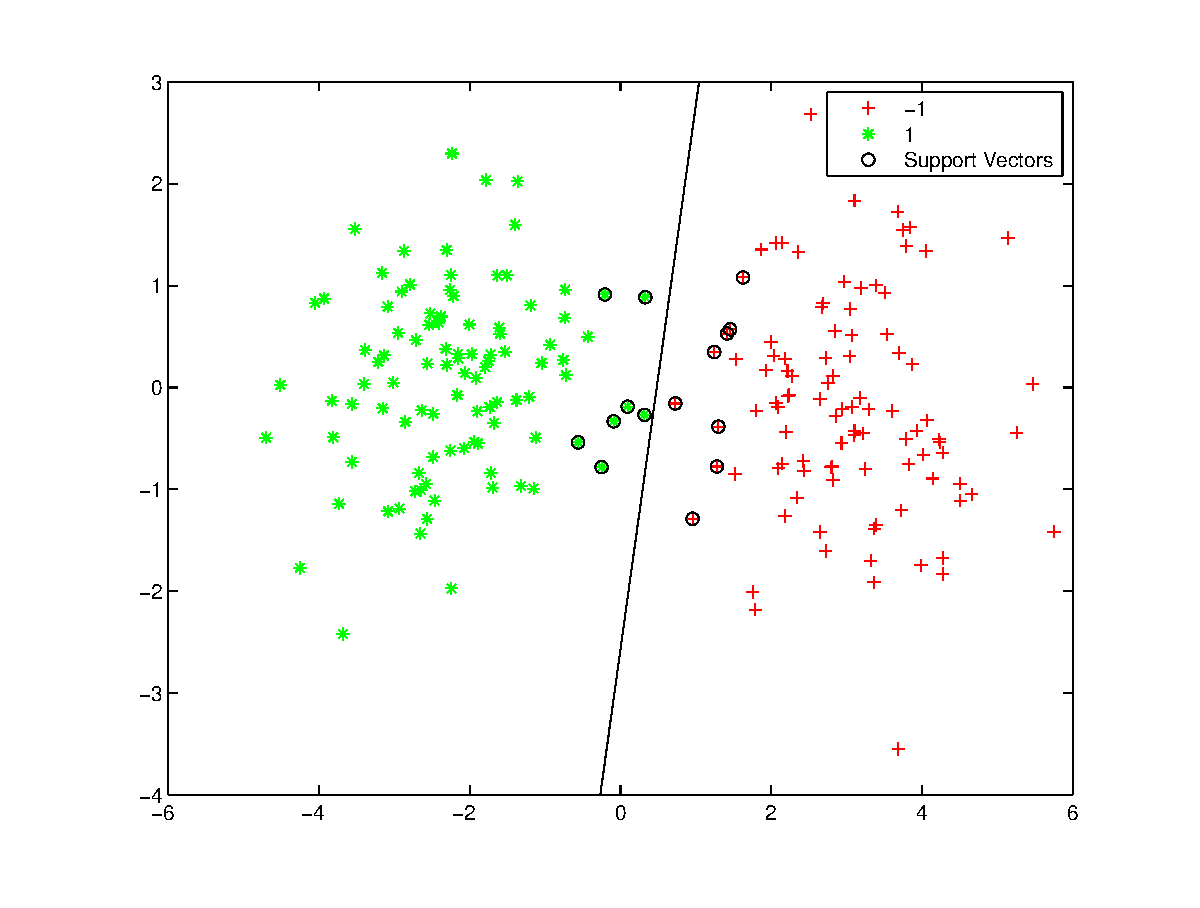
\includegraphics[width=0.5\textwidth]{figures/svm_linear_classification.eps}
            \caption{Binary classification on a dataset using a linear kernel SVM}
        \end{figure}
    \end{frame}
    
    \begin{frame}
        \frametitle{Kernel functions}
        \begin{columns}
            \visible<1->{
                \begin{column}{0.4\textwidth}
                    \begin{figure}
                        \centering
                        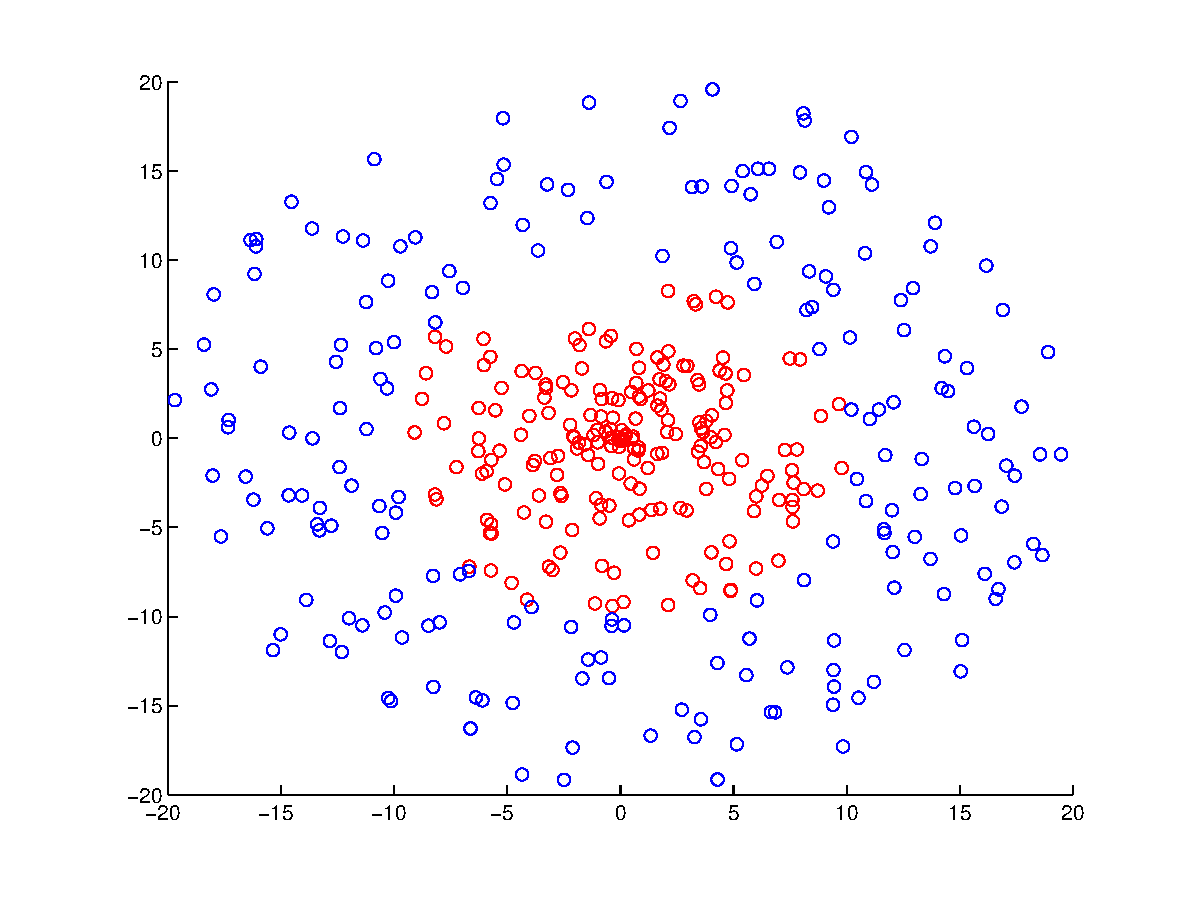
\includegraphics[width=\textwidth]{figures/svm_non_linear_data.eps}
                        \caption{Dataset in 2D (cannot be classified using a linear kernel SVM)}
                    \end{figure}
                \end{column}
            }
            \visible<2->{
                \begin{column}{0.2\textwidth}
                    \begin{center}
                        $\xrightarrow{x_3 = \sqrt{x_1^2 + x_2^2}}$
                    \end{center}
                \end{column}
            }
            \visible<3->{
                \begin{column}{0.4\textwidth}
                    \begin{figure}
                        \centering
                        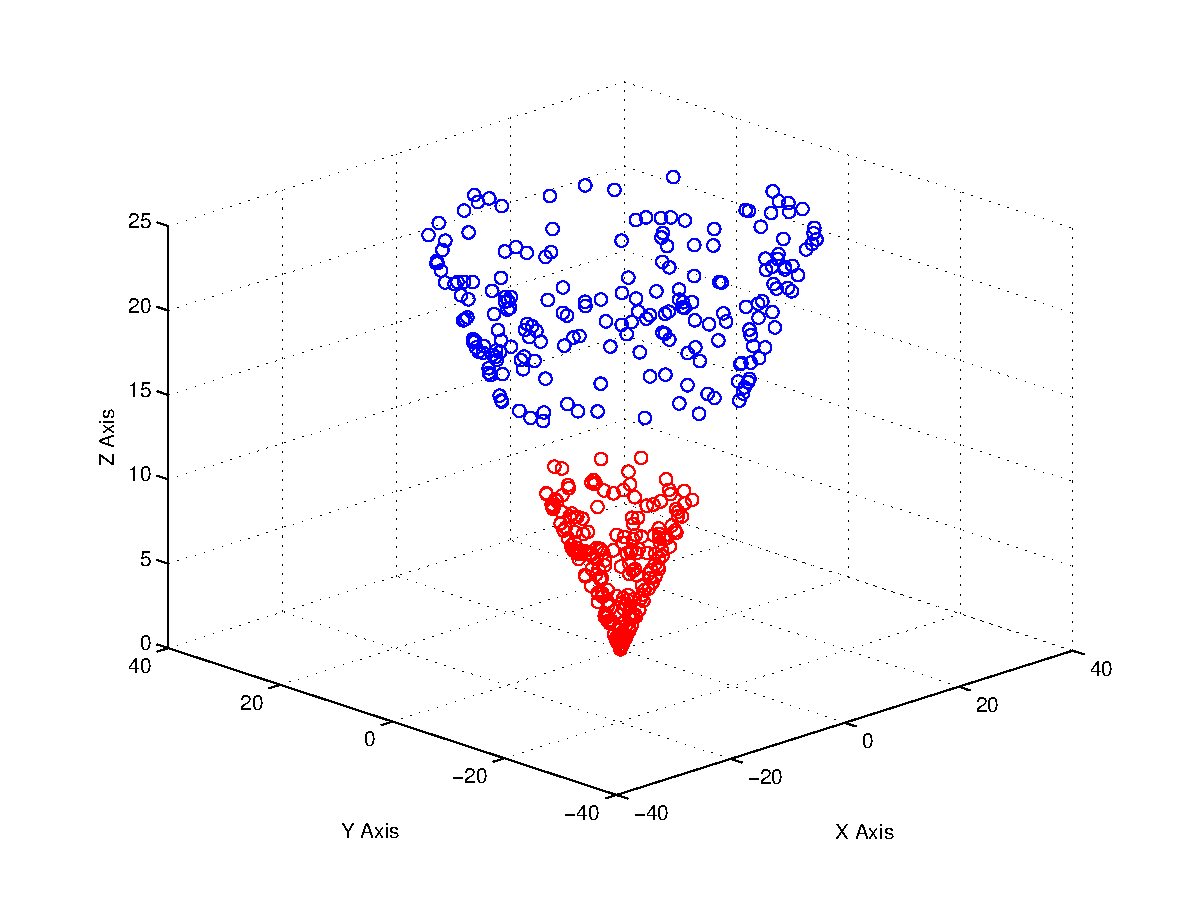
\includegraphics[width=\textwidth]{figures/svm_non_linear_data_3d.eps}
                        \caption{Dataset transformed to 3D}
                    \end{figure}
                \end{column}
            }
        \end{columns}
    \end{frame}
    
    \begin{frame}
        \frametitle{Ensemble Learning}
        \begin{itemize}
            \item{Class of machine learning methods that combine models to obtain better predictions}
            \item{Various strategies to combine models - \emph{select best}, \emph{voting (bagging)}, \emph{boosting}, \emph{stacking}}
            \pause
            \item{Performance not guaranteed to be better than constituent classifiers}
            \item{Ensemble methods still usually outperform individual classifiers}
            \item{Soft requirement - underlying models should be diverse}
        \end{itemize}
    \end{frame}
    
    \begin{frame}
        \frametitle{Bagging}
        \begin{itemize}
            \item{Obtain predictions from all constituent classifiers, and take a majority vote}
            \item{Final prediction = $\mathrm{sign}(\displaystyle \sum_{m = 1}^M y_m(\mathbf{x_n}))$}
        \end{itemize}
        \begin{columns}
            \begin{column}{0.5\textwidth}
                \[
                \begin{pmatrix}
                    x_{1,1} & x_{1,2} & x_{1, 3} & \cdots & x_{1,D} \\
                    x_{2,1} & x_{2,2} & x_{2, 3} & \cdots & x_{2,D} \\
                    x_{3,1} & x_{3,2} & x_{3, 3} & \cdots & x_{3,D} \\
                    \vdots  & \vdots  & \ddots & \vdots  \\
                    x_{N,1} & x_{N,2} & x_{N, 3} & \cdots & x_{N,D}
                \end{pmatrix}
                \]
                \begin{center}
                    \textbf{Sample split}
                \end{center}
            \end{column}
            \begin{column}{0.5\textwidth}
                \[
                \begin{pmatrix}
                    x_{1,1} & x_{1,2} & x_{1, 3} & \cdots & x_{1,D} \\
                    x_{2,1} & x_{2,2} & x_{2, 3} & \cdots & x_{2,D} \\
                    x_{3,1} & x_{3,2} & x_{3, 3} & \cdots & x_{3,D} \\
                    \vdots  & \vdots  & \ddots & \vdots  \\
                    x_{N,1} & x_{N,2} & x_{N, 3} & \cdots & x_{N,D}
                \end{pmatrix}
                \]
                \begin{center}
                    \textbf{Feature split}
                \end{center}
            \end{column}
        \end{columns}
    \end{frame}
    
    \begin{frame}
        \frametitle{Boosting}
        \begin{itemize}
            \item{Assign each sample a weight value (same for all samples in the beginning), and train $M$ classifiers successively}
            \item{For each classifier, calculate $\epsilon$ (measure of error) and $\alpha$ (decreases with $\epsilon$)}
            \item{Final prediction = $\mathrm{sign}(\displaystyle \sum_{m = 1}^{M} \alpha_m y_m(\mathbf{x_n}))$}
        \end{itemize}
        \begin{columns}
            \begin{column}{0.3\textwidth}
                \begin{center}
                    \begin{tabular}{| c |}
                        \hline
                        $\mathbf{x_1}$\\
                        \hline
                        $\mathbf{x_2}$\\
                        \hline
                        $\mathbf{x_3}$\\
                        \hline
                        $\mathbf{x_4}$\\
                        \hline
                        $\mathbf{x_5}$\\
                        \hline
                    \end{tabular}
                \end{center}
            \end{column}
            \begin{column}{0.05\textwidth}
                $\rightarrow$
            \end{column}
            \begin{column}{0.3\textwidth}
                \begin{center}
                    \begin{tabular}{| c |}
                        \hline
                        $\mathbf{x_1}$\\
                        \hline
                        $\mathbf{x_2}$\\
                        \hline
                        $\mathbf{x_3}$\\
                        \hline
                        $\mathbf{x_4}$\\
                        \hline
                        $\mathbf{x_5}$\\
                        \hline
                    \end{tabular}
                \end{center}
            \end{column}
            \begin{column}{0.05\textwidth}
                $\rightarrow$
            \end{column}
            \begin{column}{0.3\textwidth}
                \begin{center}
                    \begin{tabular}{| c |}
                        \hline
                        $\mathbf{x_1}$\\
                        \hline
                        $\mathbf{x_2}$\\
                        \hline
                        $\mathbf{x_3}$\\
                        \hline
                        $\mathbf{x_4}$\\
                        \hline
                        $\mathbf{x_5}$\\
                        \hline
                    \end{tabular}
                \end{center}
            \end{column}
        \end{columns}
    \end{frame}
    
    \begin{frame}
        \frametitle{Stacking}
        \begin{figure}
            \centering
            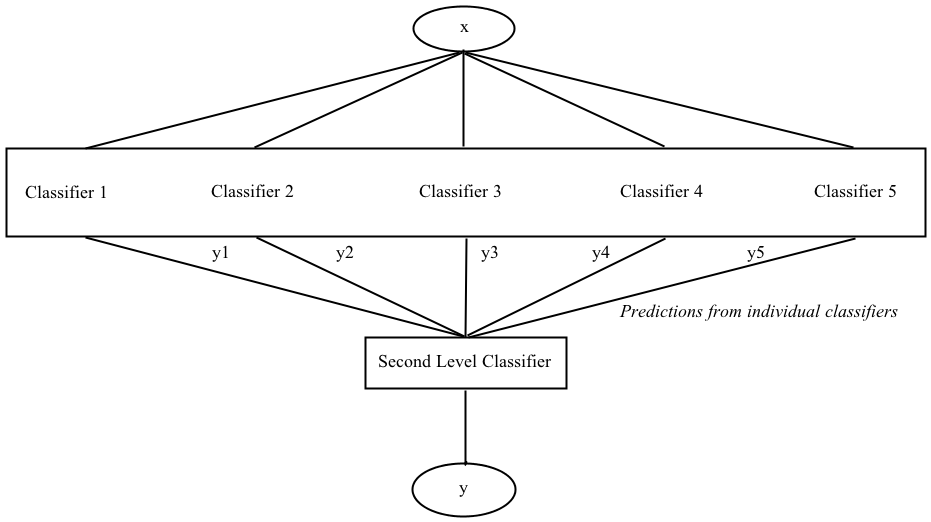
\includegraphics[width=0.7\textwidth]{figures/stacking_prediction_flow.png}
        \end{figure}
        \begin{itemize}
            \item{Outputs from first layer form the input for second layer}
            \item{Layer-1 classifiers can be trained using bootstrapping or selecting random features}
        \end{itemize}
    \end{frame}
    
    \begin{frame}
        \begin{center}
            \textbf{Experiments}
        \end{center}
    \end{frame}
    
    \begin{frame}
        \frametitle{Experiments}
        \begin{center}
            \textbf{Dataset}
        \end{center}
        \begin{itemize}
            \item{List of 6182 comments from the internet - Kaggle \footnote{\url{http://www.kaggle.com/c/detecting-insults-in-social-commentary}}}
            \item{label $|$ timestamp $|$ comment}
            \item{
            Examples
            \begin{itemize}
                \item{1 - \textcolor{red}{How arrogant you are}}
                \item{1 - \textcolor{red}{you are human garbage}}
                \item{0 - \textcolor{blue}{i really don't understand your point. It seems you are mixing apples and oranges.}}
                \item{0 - \textcolor{blue}{you may be right}}
            \end{itemize}
            }
        \end{itemize}
    \end{frame}
    
    \begin{frame}
        \frametitle{Experiments}
        \begin{center}
            \textbf{Approach}
        \end{center}
        \visible<1->{
            \begin{itemize}
                \item{Extract n-grams upto size 2 and use tf-idf information as feature values}
                \item{Input matrix - 6182 rows and 23175 columns}
                \pause
                \item{Implement all models in MATLAB}
                \item{Start with 100 samples, and continue adding 100 samples in each iteration until no more samples are left}
                \pause
            \end{itemize}
        }
        \visible<3->{
            \begin{center}
                \begin{tabular}{ | c | c | c | c | }
                    \hline
                    Name & Accuracy & Support Vector Count & Model Count\\
                    \hline
                    SVM & \ding{51} & \ding{51} & \ding{55}\\
                    Bagging & \ding{51} & \ding{55} & \ding{51}\\
                    Boosting & \ding{51} & \ding{55} & \ding{55}\\
                    Stacking & \ding{51} & \ding{55} & \ding{55}\\
                    \hline
                \end{tabular}
            \end{center}
        }
    \end{frame}
    
    \begin{frame}
        \frametitle{Experiments}
        \begin{center}
            \textbf{Support Vector Machines}
        \end{center}
        \begin{columns}
            \begin{column}{0.5\textwidth}
                \begin{figure}
                    \centering
                    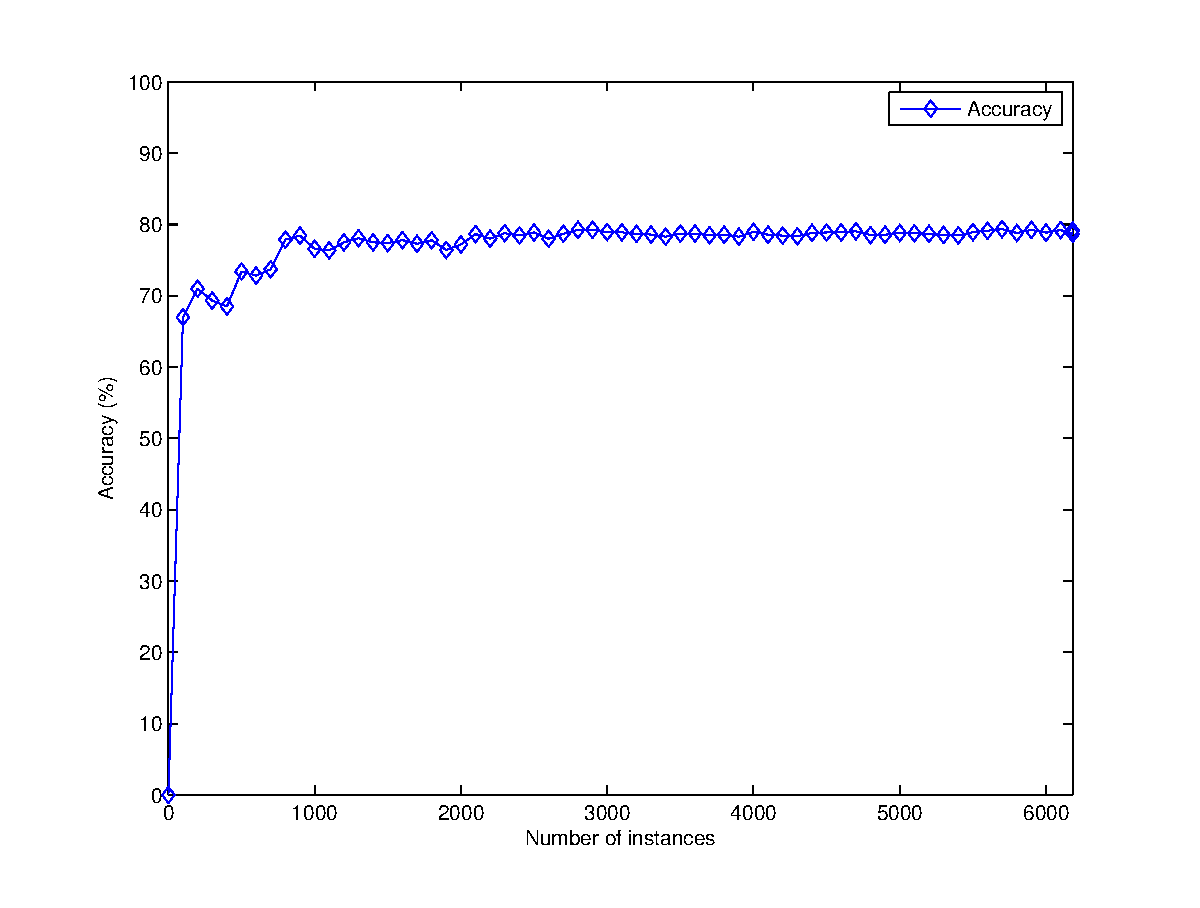
\includegraphics[width=\textwidth]{figures/svm_accuracy.eps}
                    \caption{Accuracy}
                \end{figure}
                \begin{center}
                    \small 79.02\% for linear kernel, and 34.39\% for Polynomial/RBF/Sigmoid kernels
                \end{center}
            \end{column}
            \begin{column}{0.5\textwidth}
                \begin{figure}
                    \centering
                    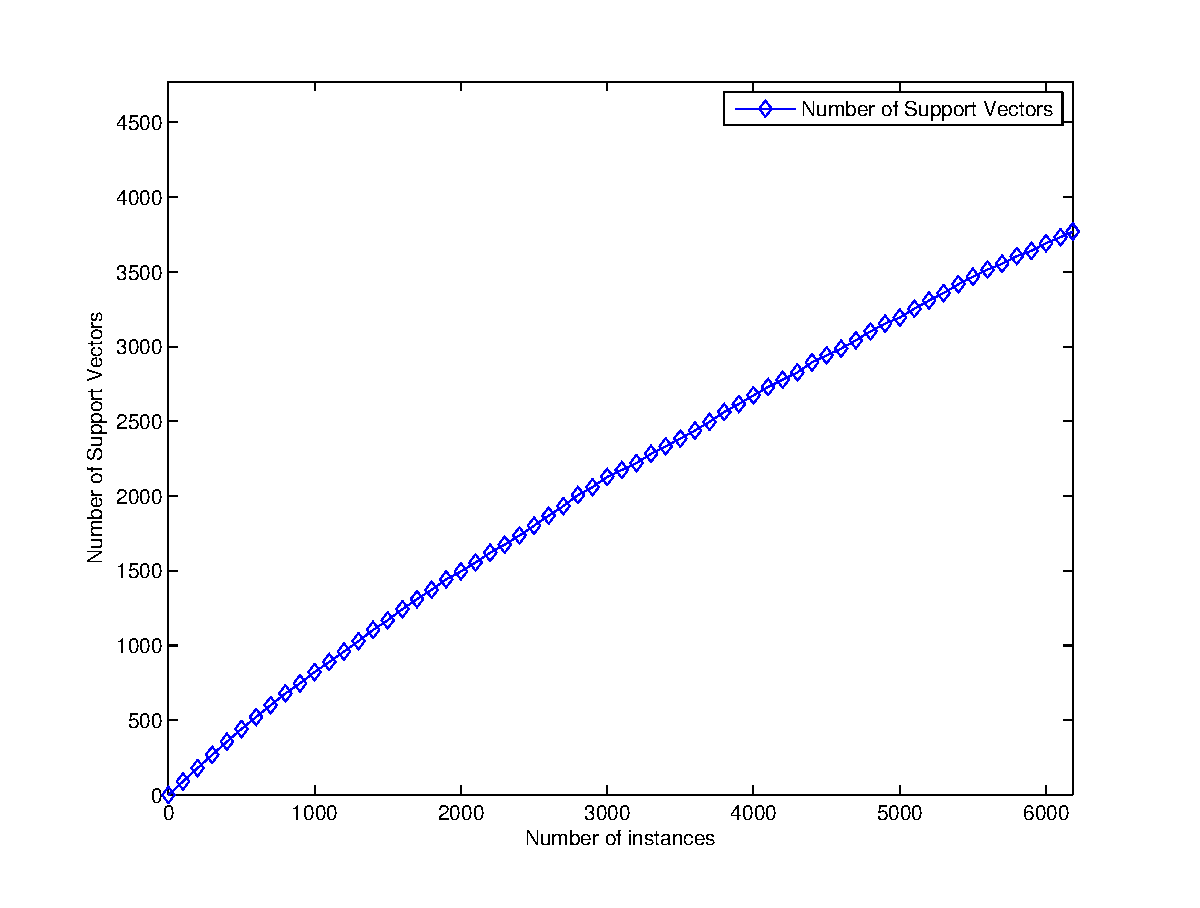
\includegraphics[width=\textwidth]{figures/svm_n_sv.eps}
                    \caption{Support Vector count}
                \end{figure}
                \begin{center}
                    \small Number of support vectors decreases from 90\% to 60\%
                \end{center}
            \end{column}
        \end{columns}
    \end{frame}
    
    \begin{frame}
        \frametitle{Experiments}
        \begin{center}
            \textbf{Bagging}
        \end{center}
        \begin{columns}
            \begin{column}{0.5\textwidth}
                \begin{figure}
                    \centering
                    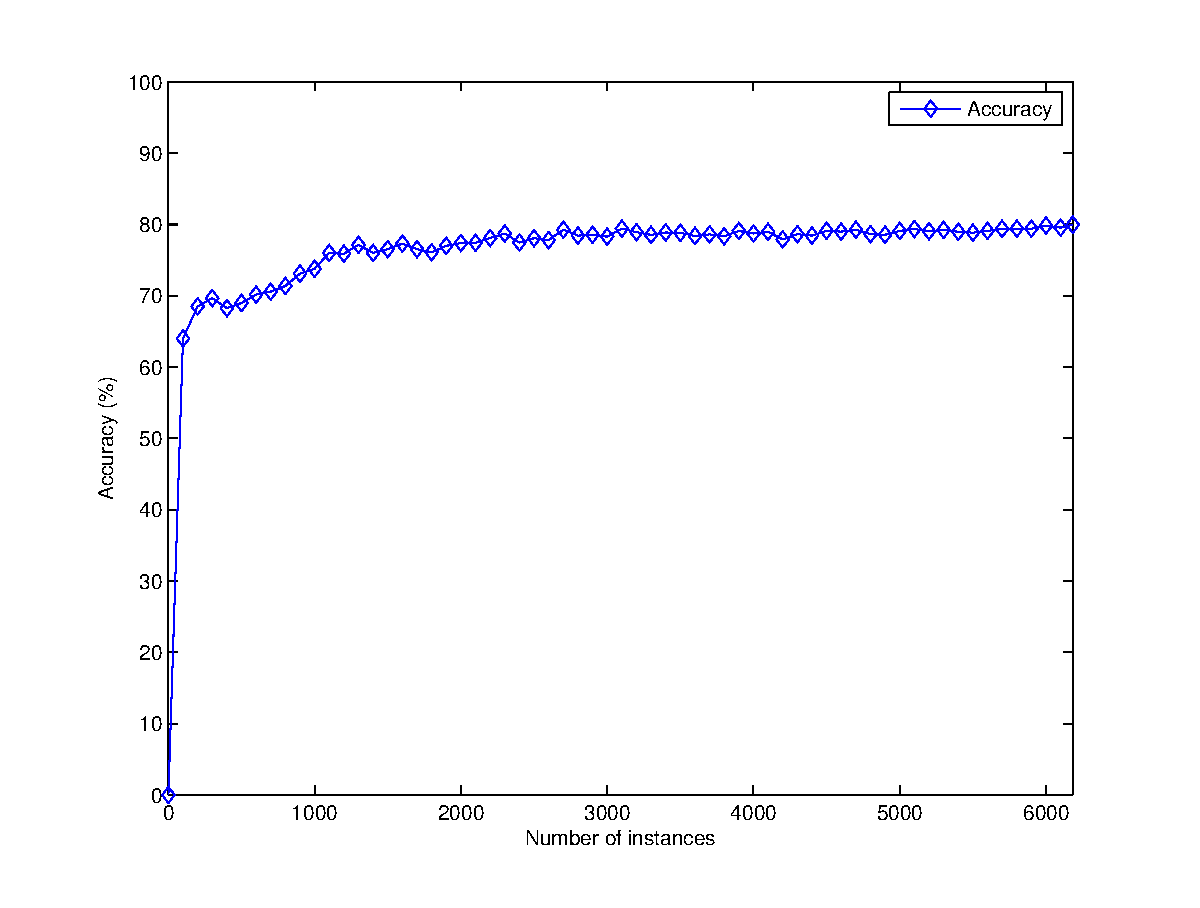
\includegraphics[width=\textwidth]{figures/bagging_accuracy.eps}
                    \caption{Accuracy v/s Number of instances}
                \end{figure}
                \begin{center}
                    \small 79.65\% (9 linear kernel SVMs)
                \end{center}
            \end{column}
            \begin{column}{0.5\textwidth}
                \begin{figure}
                    \centering
                    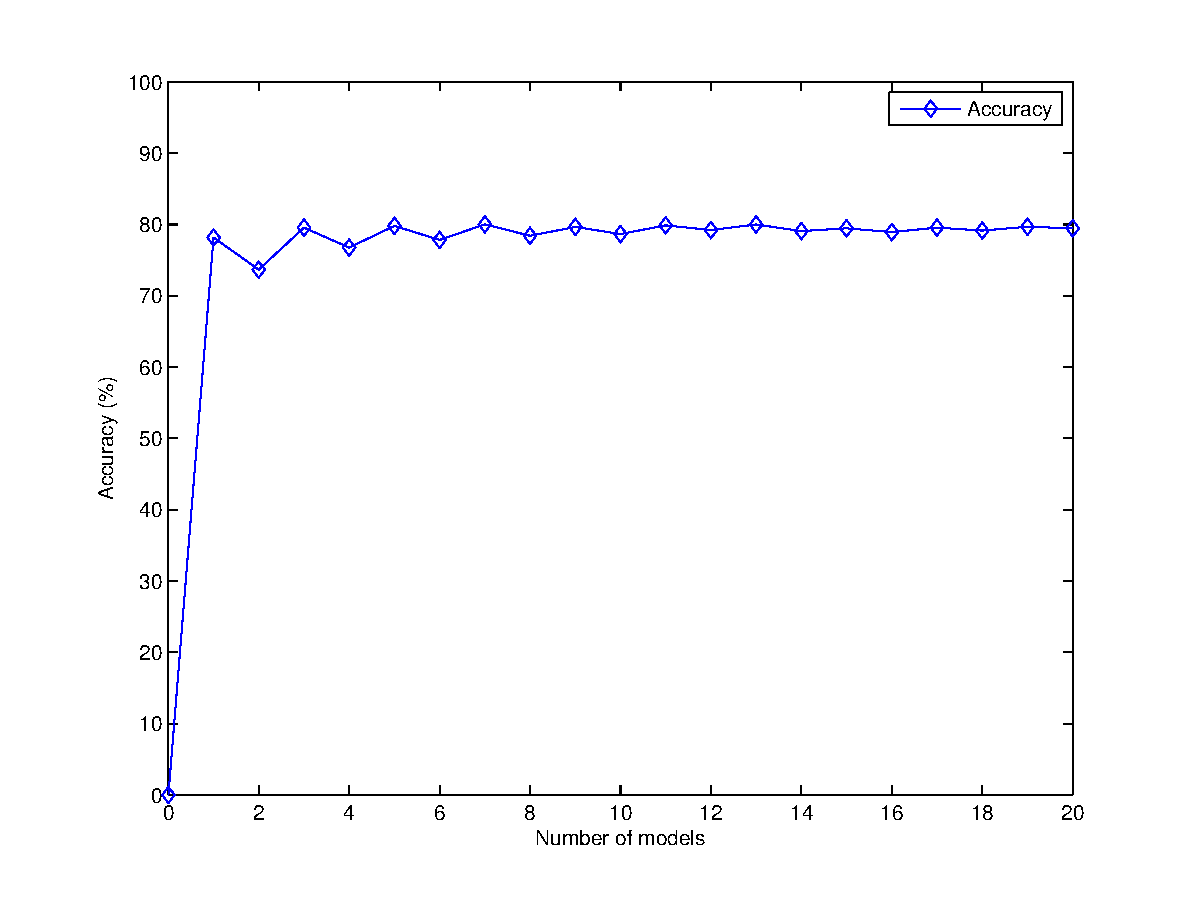
\includegraphics[width=\textwidth]{figures/bagging_n_models.eps}
                    \caption{\small Accuracy v/s Number of models}
                \end{figure}
                \begin{center}
                    \small Models increase $\rightarrow$ Subsets overlap $\rightarrow$ Accuracy Stabilizes
                \end{center}
            \end{column}
        \end{columns}
    \end{frame}
    
    \begin{frame}
        \frametitle{Experiments}
        \begin{columns}
            \begin{column}{0.5\textwidth}
                \begin{center}
                    \textbf{Boosting}
                \end{center}
                \begin{figure}
                    \centering
                    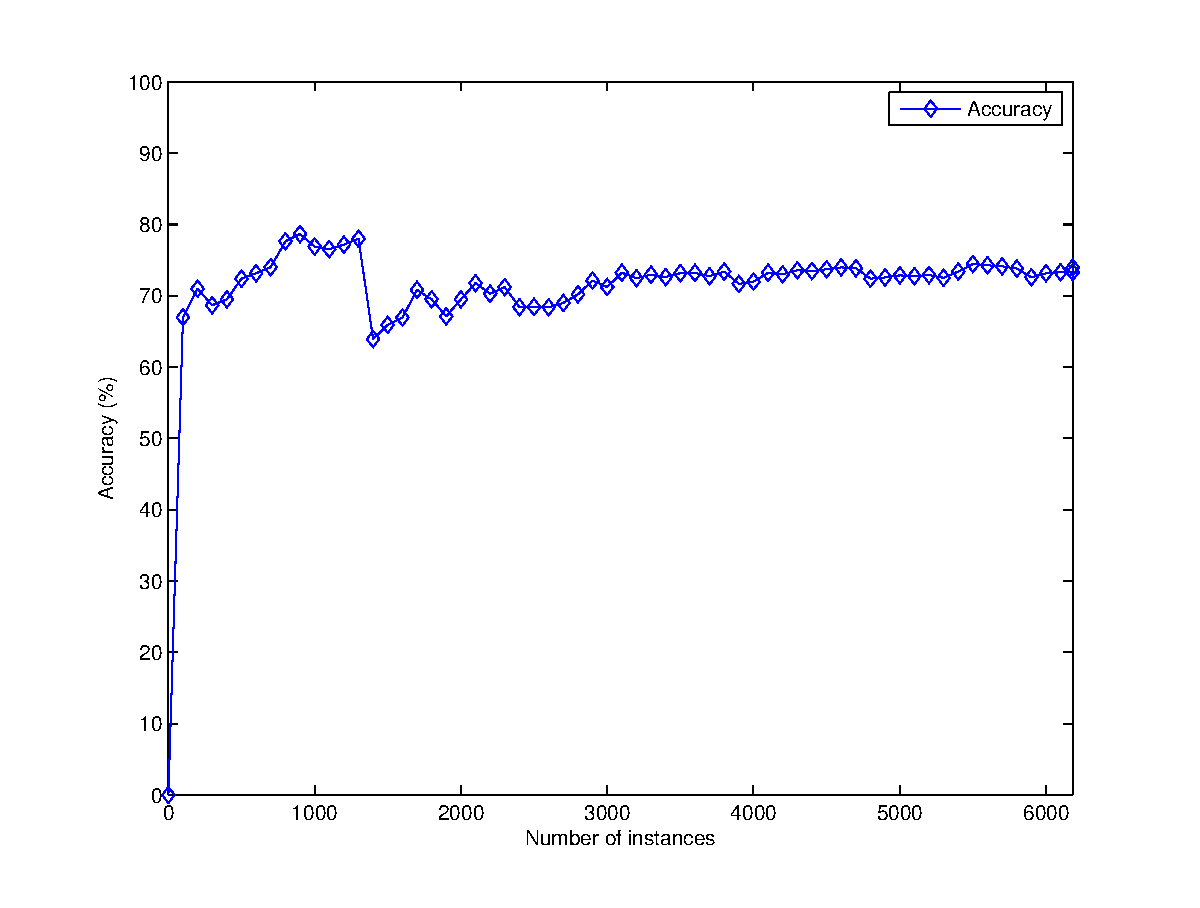
\includegraphics[width=\textwidth]{figures/boosting_accuracy.eps}
                \end{figure}
                \begin{center}
                    Average accuracy of 72.84\%
                \end{center}
            \end{column}
            \begin{column}{0.5\textwidth}
                \begin{center}
                    \textbf{Stacking}
                \end{center}
                \begin{figure}
                    \centering
                    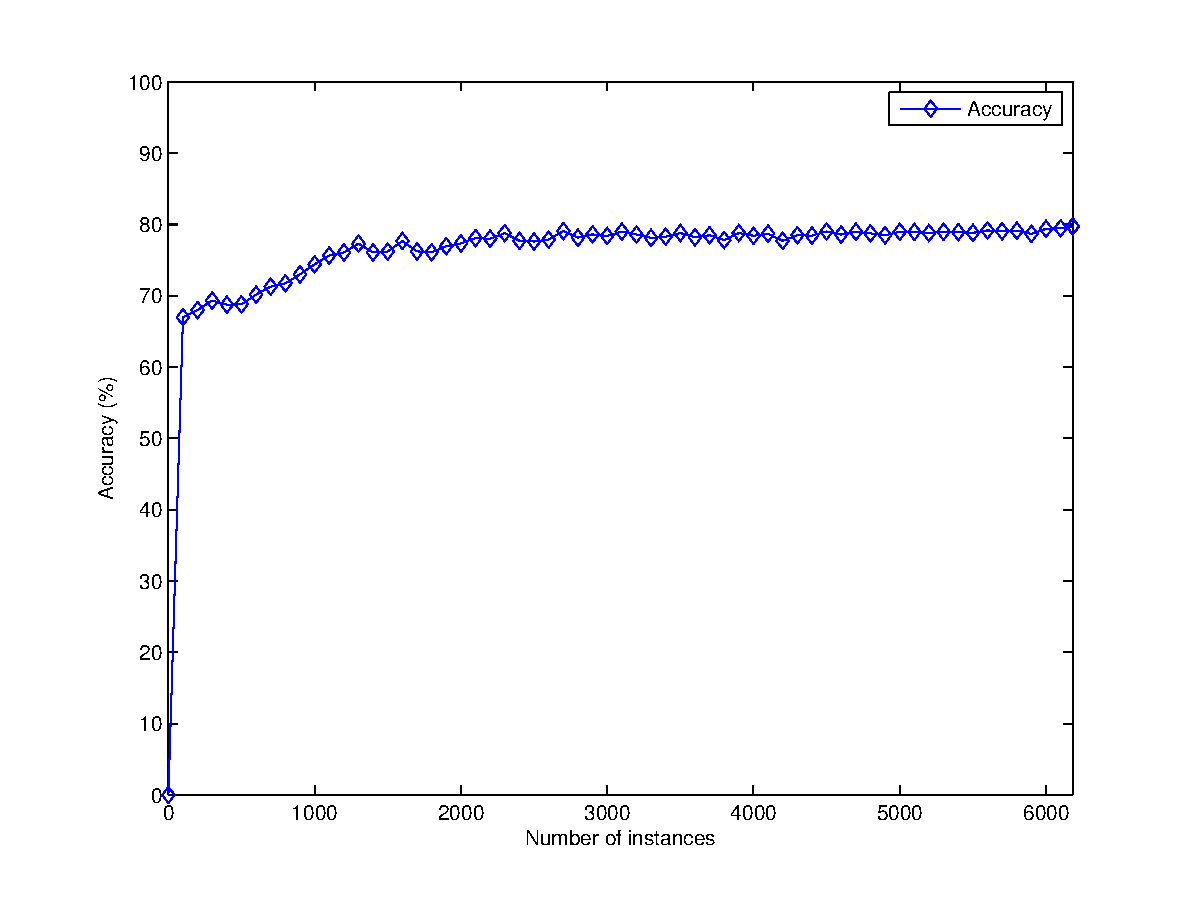
\includegraphics[width=\textwidth]{figures/stacking_accuracy.eps}
                \end{figure}
                \begin{center}
                    Average accuracy of 79.48\%
                \end{center}
            \end{column}
        \end{columns}
        \begin{center}
            All using linear kernel SVMs
        \end{center}
    \end{frame}
    
    \begin{frame}
        \begin{center}
            \textbf{System}
        \end{center}
    \end{frame}
    
    \begin{frame}
        \frametitle{System}
        \begin{center}
            \textbf{Dataset}
        \end{center}
        \visible<1->{
            \begin{itemize}
                \item{\textbf{Training data} - Reddit}
                \item{Fetch posts from ``/r/happy'' \footnote{\url{http://www.reddit.com/r/happy}} and ``/r/suicidewatch'' \footnote{\url{http://www.reddit.com/r/suicidewatch}}}
                \pause
                \item{\textbf{Prediction data} - Twitter}
                \item{Gather tweets from the public streaming API \footnote{\url{https://dev.twitter.com/docs/streaming-apis/streams/public}}}
                \pause
            \end{itemize}
        }
        \visible<3->{
            \begin{center}
                \begin{tabular}{ | c | c | }
                    \hline
                    \textbf{Task} & \textbf{Frequency} \\
                    \hline
                    Fetch 1000 posts from Reddit & 24 hours \\
                    Fetch 100 tweets from Twitter & 3 hours \\
                    Re-assign labels to previous tweets and update statistics & 24 hours \\
                    \hline
                \end{tabular}
            \end{center}
        }
    \end{frame}
    
    \begin{frame}
        \frametitle{System}
        \begin{center}
            \textbf{Approach}
        \end{center}
        \begin{itemize}
            \item{Implement all classifiers in Python, and web interface in Django}
            \item{No training data available $\rightarrow$ build our own}
            \pause
            \item{
            Training data (Reddit)
            \begin{itemize}
                \item{``/r/happy'' - people posts their happy moments}
                \item{``/r/suicidewatch'' - people post when they want to commit suicide}
                \item{labels assigned by users of our system}
            \end{itemize}
            }
            \pause
            \item{
            Prediction data (Twitter)
            \begin{itemize}
                \item{General sentiment of the overall public}
                \item{Pull 100 tweets every 3 hours from Twitter}
            \end{itemize}
            }
        \end{itemize}
    \end{frame}
    
    \begin{frame}
        \frametitle{System}
        \begin{center}
            \textbf{Architecture}
        \end{center}
        \begin{columns}
            \begin{column}{0.5\textwidth}
                \begin{figure}
                    \centering
                    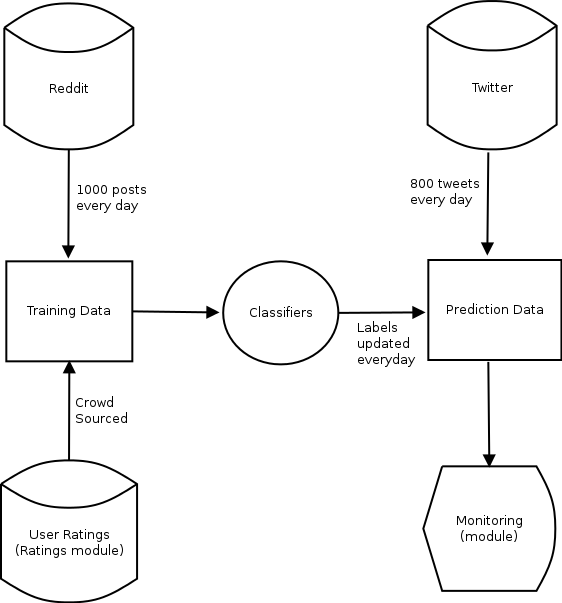
\includegraphics[width=\textwidth]{figures/Architecture.png}
                \end{figure}
            \end{column}
            \begin{column}{0.5\textwidth}
                \begin{itemize}
                    \item{\textbf{Ratings} - allows users to assign labels to stories (crowd intelligence), building the training data}
                    \item{\textbf{Monitoring} - displays predictions of classifiers in the form of depressed tweets and individual statuses of classifiers}
                \end{itemize}
            \end{column}
        \end{columns}
    \end{frame}
    
    \begin{frame}
        \begin{center}
            \textbf{Demo}
        \end{center}
    \end{frame}
    
    \begin{frame}
        \begin{center}
            \textbf{Conclusion and Future Work}
        \end{center}
    \end{frame}
    
    \begin{frame}
        \frametitle{Conclusion}
        \begin{itemize}
            \item{An evaluation of Support Vector Machines and Ensemble Learning methods (Bagging/Boosting/Stacking) in the domain of text classification}
            \item{Bagging outperformed Stacking outperformed SVM outperformed Boosting}
            \pause
            \item{A web based system that can detect emotional distress on Twitter}
            \item{No labels implies qualitative evaluation is difficult except observation}
            \item{Observed results seem to be reasonable}
        \end{itemize}
    \end{frame}
    
    \begin{frame}
        \frametitle{Future Work}
        \begin{itemize}
            \item{Fetch more tweets}
            \item{Increase the crowd intelligence involved}
            \pause
            \item{Relabelling process (decreases wastage of resources)}
            \pause
            \item{Select best performing model}
            \item{Store confidence values}
        \end{itemize}
    \end{frame}
    
    \begin{frame}
        \begin{center}
            \textbf{Thank you!}
        \end{center}
        \begin{center}
            \textbf{Questions?}
        \end{center}
    \end{frame}
\end{document}
